\documentclass{beamer}

\usepackage[utf8]{inputenc}
\usepackage[russian]{babel}
\usepackage{cmap}

\mode<presentation> {
\usetheme{Madrid}
\setbeamertemplate{caption}[numbered]
}

\usepackage{graphicx} % Allows including images
\usepackage{booktabs} % Allows the use of \toprule, \midrule and \bottomrule in tables

\title[Интеллектуальные системы]{Задача выделения объекта на изображении: хаотично-фазовая синхронизация и асинхронность в осцилляторных нейронных сетях}

\author{Мартынов Семён}
\institute[СПб ПУ]
{
Санкт-Петербургский государственный политехнический университет \\
\medskip
\textit{semen.martynov@gmail.com}
}
\date{\today}

\begin{document}

\begin{frame}
\titlepage
\end{frame}

\begin{frame}
\frametitle{Содержание}
\tableofcontents
\end{frame}

%------------------------------------------------
\section{Базовые понятия}
%------------------------------------------------

\begin{frame}
\frametitle{Базовые понятия}
\begin{block}{Нейронная сеть (1)}
Сложная совокупность нейронов, функционально объединенных в нервной системе и обеспечивающих взаимосвязанное поведение всех систем организма.
\end{block}

\begin{block}{Нейронная сеть (2)}
Упрощенная (математическая/программная/аппаратная) модель биологической нейронной сетей.
\end{block}

\begin{block}{Осцилляторная нейронная сеть}
Класс нейронных сетей, в котором рассматриваются колебательные аспекты их функционирования. Функциональной единицей осцилляторных нейронных сетей, как правило, является \underline{осциллятор},\\т. е. объект с колебательными свойствами. 
\end{block}
\end{frame}

%------------------------------------------------
\section{Синхронизация и зрительное внимание}
%------------------------------------------------

\begin{frame}
\frametitle{Синхронизация и зрительное внимание}

Какие объекты находятся на рисунке 1?

\begin{figure}
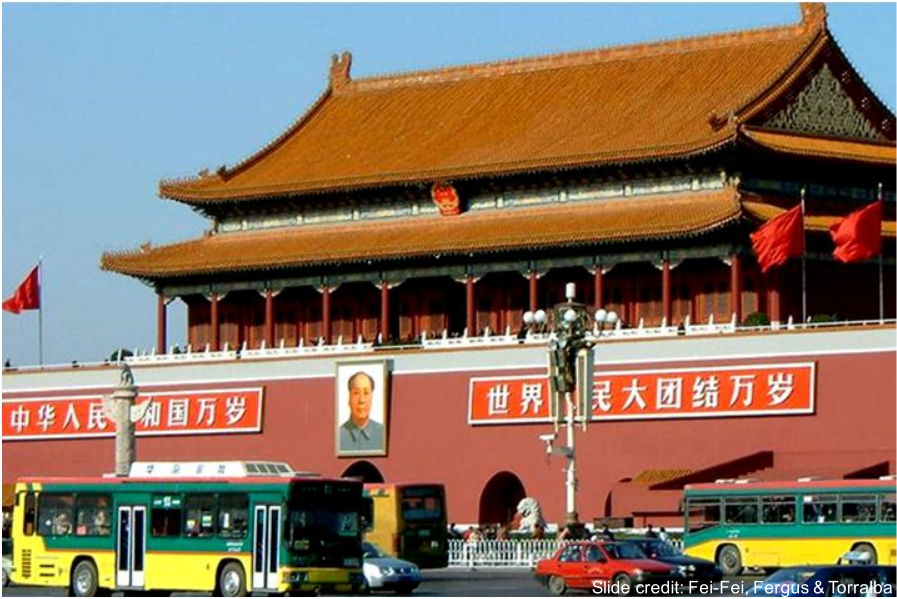
\includegraphics[scale=0.35]{img/tiananmen_square}
\caption{Площадь Тяньаньмэнь}
\end{figure}

\end{frame}

%------------------------------------------------

\begin{frame}
\frametitle{Синхронизация и зрительное внимание}

Что позволяет их выделить объекты на рисунке 2?

\begin{figure}
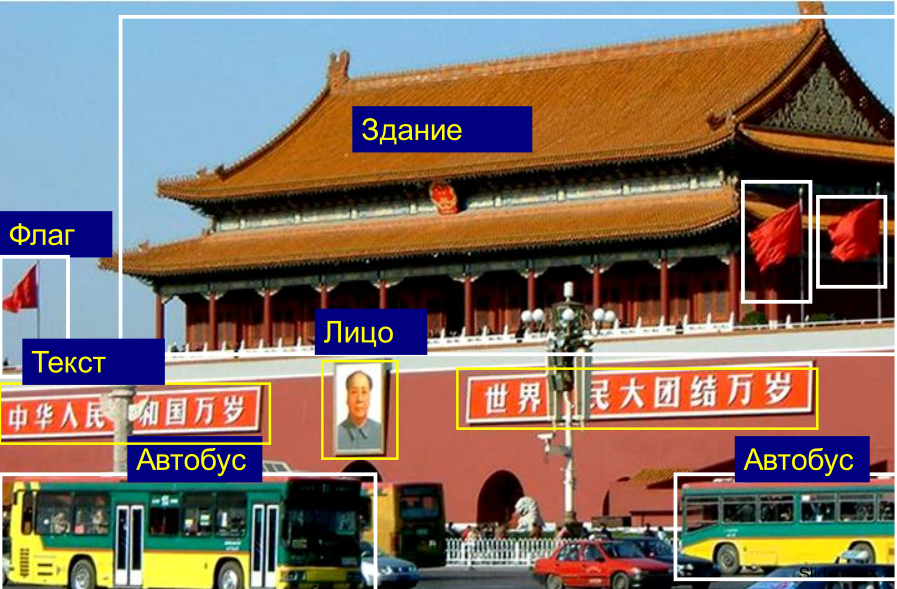
\includegraphics[scale=0.35]{img/tiananmen_square2}
\caption{Площадь Тяньаньмэнь с выделенными объектами}
\end{figure}

\end{frame}

%------------------------------------------------

\begin{frame}
\frametitle{Синхронизация и зрительное внимание}

Идея динамического связывания (dynamical binding):

\begin{itemize}
\item Колебательная нейронная активность и синхронизация в зрительной коре мозга кошки и обезьяны.
\item Использования явлений синхронизации и резонанса в других структурами мозга (обонятельной корой, гиппокампом, таламокортикальной системой, новой корой).
\end{itemize}
\pause
В отличие от медленной адаптации нейронных сетей под действием алгоритмов обучения, динамическое связывание способно обеспечить \textit{немедленную} реакцию сети, необходимую при выполнении задач обработки информации в режиме реального времени!

\end{frame}

%------------------------------------------------

\begin{frame}
\frametitle{Синхронизация и зрительное внимание}

Существуют два базовых подхода к построению компьютерной модели формирования внимания:
\begin{itemize}
\item[-] на основе места (location-based model) - активируется одним (сигнальным) нейроном, акцент на одну точку;
\item[-] на основе объекта (object-based model) - базовым юнитом, конкурирующим за внимание является целый объект (либо его часть).
\end{itemize}
\pause
Биологические системы обучились вычленять из окружающей среды максимально релевантную информацию (WTA), и подавлять второстепенную. Объект, захвативший внимание, постепенно теряет \textit{актуальность}, уступая остальным объектам.

\end{frame}

%------------------------------------------------

\begin{frame}
\frametitle{Синхронизация и зрительное внимание}

\begin{itemize}
\item[]Благодаря связи между синхронизацией и зрительным вниманием, были предложены модели распознавания объектов с полной синхронизация между осцилляторами, используемыми для представления объектов.
\bigskip
\pause
\item[]На практике, феномен полной синхронизации встречался крайне редко.
\bigskip
\pause
\item[]Следовательно, прочие формы синхронизации должны быть рассмотрены! 
\end{itemize}

\end{frame}

%------------------------------------------------

\begin{frame}
\frametitle{Синхронизация и зрительное внимание}

Виды синхронизаций:

\begin{itemize}
\item Полная (complete synchronization) -  полная сходимость (во времени) соответствующих переменных всех нейронов в сети.
\item Фазовая (phase synchronization) - разность фаз между элементами сети со временем должна либо вообще не меняться, либо находиться в определённых конечных границах, при этом игнорируя отношение амплитуд.
\item Запаздывающая (lag synchronization) - происходит в сильно связных колебательных системах, когда они выровняются по фазе и амплитуде, но остаются сдвинуты во времени.
\item Опережающая (anticipating synchronization) - происходит в сонаправленных системах коллективного поведения, где одна система движется с определением относительно остальных.
\item Обобщенная (generalized synchronization) - подобна фазовой, только отношение между фазами должны описываться определённой функцией.
\end{itemize}

\end{frame}


%------------------------------------------------
\section{Хаотично-фазовая синхронизация}
%------------------------------------------------

\begin{frame}
\frametitle{Хаотично-фазовая синхронизация}

\begin{itemize}
\item[]Подход фазовой синхронизации позволяет исследовать синхронизацию сетей с осцилляторами, параметры которых могут отличаться.
\bigskip
\item[]Рассмотрим \underline{хаотично-фазовую синхронизацию} на основе \underline{сдвоенного хаотического аттрактора Рёсслера}, которая позволяет создать механизм поиска и \textit{подсветки} объекта, на который будет обращено внимание.
\bigskip
\item[]В процессе работы, группа нейронов (представляющих приметный объект на снимке) фиксируется по своей фазе, т.е. каждый нейрон производит уникальную хаотическую траекторию, но вместе они оказываются фазной-связанными. В это же время, другие группы нейронов, представляющие другие объекты на снимке, двигаются в своих фазах, никак не связанных с рассматриваемой нами.
\end{itemize}

\end{frame}

%------------------------------------------------
\subsection{Аттрактор Рёсслера} % A subsection can be created just before a set of slides with a common theme to further break down your presentation into chunks

\begin{frame}
\frametitle{Хаотично-фазовая синхронизация}

\begin{itemize}
\item[]Аттрактор - компактное подмножество фазового пространства динамической системы, все траектории из некоторой окрестности которого стремятся к нему при времени, стремящемся к бесконечности.
\bigskip
\item[]Аттрактор Рёсслера — хаотический аттрактор, которым обладает система дифференциальных уравнений Рёсслера:

\begin{center}
$\left \{ \begin{matrix} \frac{dx}{dt} = -y - z \\ \frac{dy}{dt} = x + ay \\ \frac{dz}{dt} = b + z(x-c) \end{matrix} \right.  ;$
\end{center}

где $a, b, c$  — положительные постоянные. При значениях параметров $a = b = 0,2$ и $2,6 \le c \le 4,2$ уравнения Рёсслера обладают устойчивым предельным циклом. При этих значениях параметров период и форма предельного цикла совершают последовательность удвоения периода.
\end{itemize}

\end{frame}

%------------------------------------------------

\begin{frame}
\frametitle{Синхронизация и зрительное внимание}


Сразу же за точкой c = 4,2 возникает явление хаотического аттрактора. Чётко определённые линии предельных циклов расплываются и заполняют фазовое пространство бесконечным счетным множеством траекторий, обладающим свойствами фрактала.

\begin{figure}
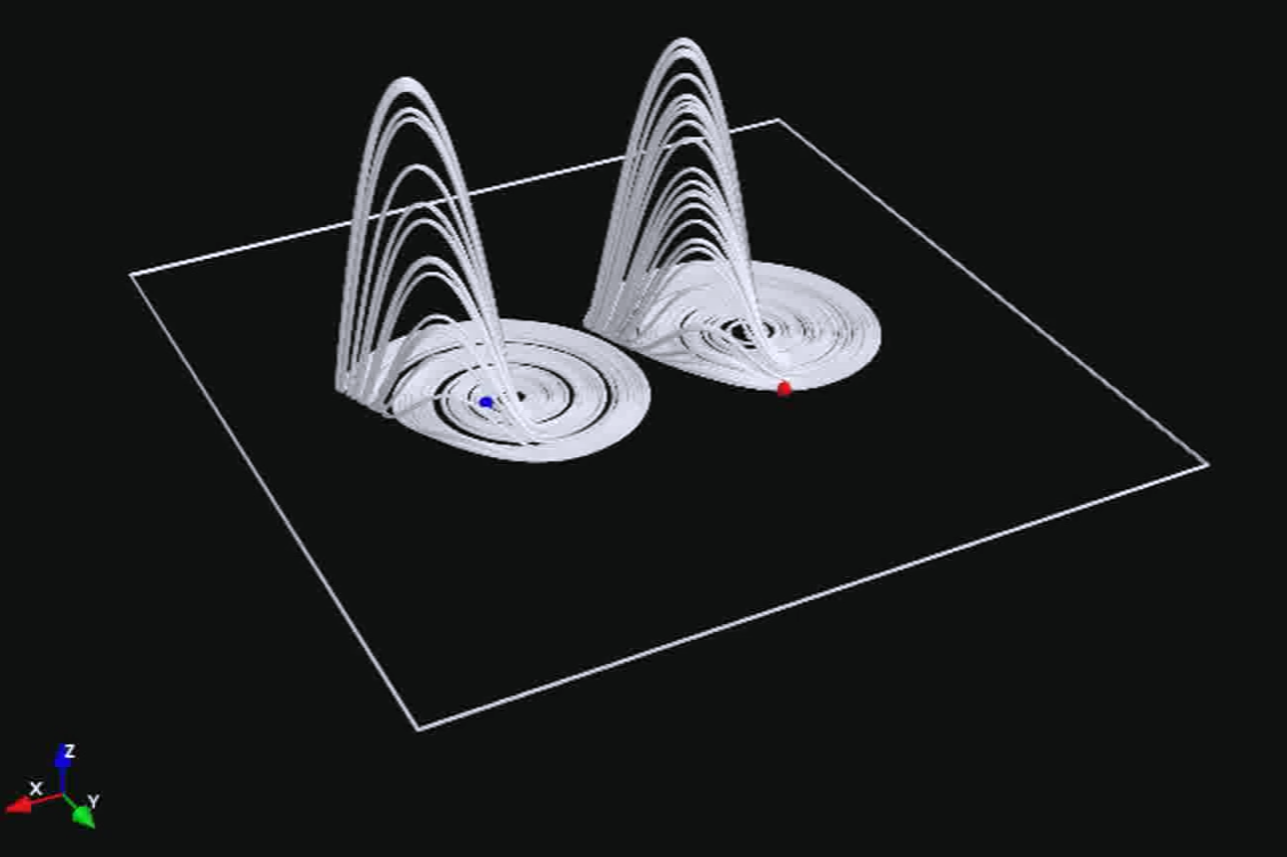
\includegraphics[scale=0.10]{img/rossler}
\caption{Сдвоенный хаотический аттрактора Рёсслера}
\end{figure}

Рекомендую видео: \url{http://www.youtube.com/watch?v=ef3M0n8MK-0}

\end{frame}
%------------------------------------------------

\begin{frame}
\frametitle{Хаотично-фазовая синхронизация}

\begin{itemize}
\item[]Два осциллятора будем называть синхронными по фазе, если разность их фаз остаётся ограниченной, а амплитуда может не коррелировать.
\bigskip
\item[] Другими словами, $|\phi_1 - \phi_2| < M$ при $t \to \infty$
\item[] Фаза осциллятора $\phi$ определяется следующим образом:
\begin{center}
$\phi = \Upsilon (\arctan (y/x))$,
\end{center}
где $x$ и $y$ являются переменными осциллятора, а функция $\Upsilon$ гарантирует рост числа $\phi$.
\end{itemize}

\end{frame}

%------------------------------------------------

\begin{frame}
\frametitle{Хаотично-фазовая синхронизация}

\begin{itemize}
\item[]Два связных осциллятора Рёсслера также могут быть синхронными по фазе, если обеспечивается достаточная \textit{сила} связности!
\bigskip
\item[] Массив из $N$ (попарно) связных осцилляторов Рёсслера представлен следующим уравнением:
\begin{center}
$\dot{x_i} = -\omega_iy_i - z_i +k(2x_i - x_{i-1} - x_{i+i})$,\\
$\dot{y_i} = \omega_ix_i - ay_i$,\\
$\dot{z_i} = b + z_i(x_i - c)$,
\end{center}
где используются три константы $a=0,15$, $b=0,2$ и $c=10$, а значение $\omega_i$ для каждого осциллятора выбирается случайным образом в интервале $[0,98 1,02]$. Параметр $k$ отвечает за \textit{силу} связности.
\end{itemize}

\end{frame}

%----------------------------------------------

\begin{frame}
\frametitle{Хаотично-фазовая синхронизация}

Возьмём 50 связных Рёсслеровских систем, и проследим по рисунку 4 переход от хаотического к синхронному состоянию. 

\begin{figure}
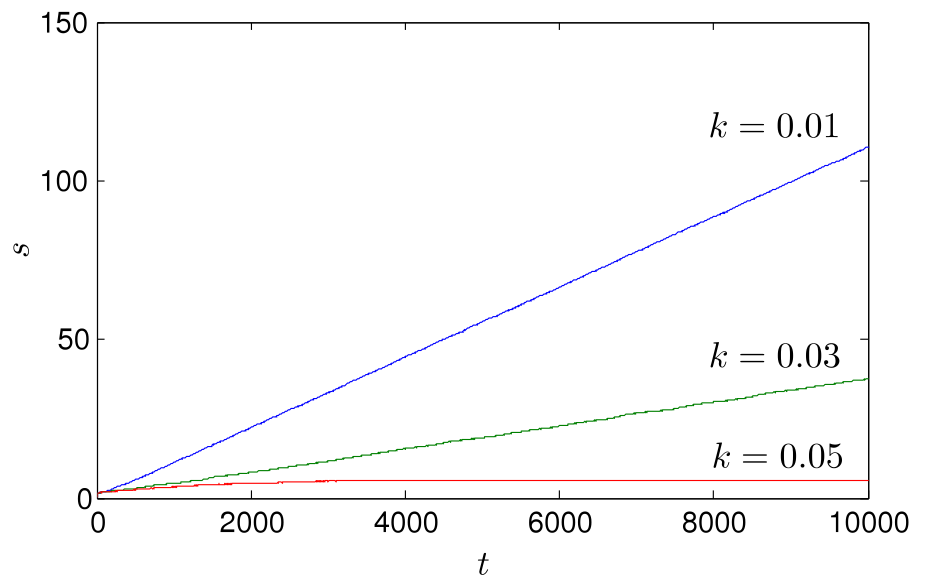
\includegraphics[scale=0.25]{img/phase_standard_deviation}
\caption{Отклонение от фазы в секундах (s) синхронной (k = 0,05), почти синхронной (k = 0,03) и не синхронной (k = 0,01) систем.}
\end{figure}

\end{frame}


%----------------------------------------------

\begin{frame}
\frametitle{Хаотично-фазовая синхронизация}

Если опустить дополнительные математические подробности (основанные на экспоненте Ляпунова), то:

\begin{itemize}
\item при силе связи равной нулю, синхронизации (в том числе фазовой синхронизации) не наблюдается.
\medskip
\item при увеличении силы связи, фазы синхронизируются, но амплитуды двух осцилляторов остаются некоррелированными.
\medskip
\item при дальнейшем росте силы связи, достигается полная синхронизация (с небольшой разницей между траекториями двух осцилляторов).
\end{itemize}

\end{frame}

%------------------------------------------------
\section{Осцилляторные сети и распознавание}
%------------------------------------------------

\begin{frame}
\frametitle{Осцилляторные сети и распознавание}

\begin{itemize}
\item[]Рассмотрим модель двухмерной сети Рёсслеровских осцилляторов, построенной по следующим формулам
\begin{center}
$\dot{x}_{i,j} = -\omega_{i,j}y_{i,j} - z_{i,j} + k^{+}_{i,j}\Delta^{+}x_{i,j} + k^{-}_{i,j}\Delta^{-}x_{i,j}$,\\
$\dot{y}_{i,j} = \omega_{i,j}x_{i,j} - ay_{i,j}$,\\
$\dot{z}_{i,j} = b + z_{i,j}(x_{i,j} - c)$,
\end{center}
где:
\item[] $(i, j)$ это решётка $1 \le i \le N, 1 \le j \le M$,
\item[] $k^{+}_{i,j} \in [0, k^{+}_{max}]$ и $k^{-}_{i,j} \in [0, k^{-}_{max}]$ положительная и отрицательная сила связывания (уст. в соответ. с пиксельными константами),
\item[] $\omega_{i,j}$ также определяется пиксельными константами,
\item[] $k^{+}_{max}$ и $k^{-}_{max}$ выбираются в зависимости от изображения,
\item[] $\Delta^{+}x_{i,j}$ и $\Delta^{-}x_{i,j}$ положительные и отрицательные условия связывания.
\end{itemize}

\end{frame}

%------------------------------------------------

\begin{frame}
\frametitle{Осцилляторные сети и распознавание}

\begin{itemize}
\item[]Положительные и отрицательные условия связывания определяются следующим образом:
\begin{center}
\begin{eqnarray*}
\Delta^{\pm}x_{i,j} &=& \gamma_{i-1,j-1;i,j}(x_{i-1,j-1}-x_{i,j}) + \gamma_{i-1,j;i,j}(x_{i-1,j}-x_{i,j}) \\
                   && + \gamma_{i-1,j+1;i,j}(x_{i-1,j+1}-x_{i,j}) + \gamma_{i,j-1;i,j}(x_{i,j-1}-x_{i,j}) \\
                   && + \gamma_{i,j+1;i,j}(x_{i,j+1}-x_{i,j}) + \gamma_{i+1,j-1;i,j}(x_{i+1,j-1}-x_{i,j}) \\
                   && + \gamma_{i+1,j;i,j}(x_{i+1,j}-x_{i,j}) + \gamma_{i+1,j+1;i,j}(x_{i+1,j+1}-x_{i,j}),
\end{eqnarray*}
\end{center}
\item[] где
\begin{center}
	$$
	\gamma_{i,j;p,q} = \left\{ \begin{array}{rl}
	 1, &\mbox{ если осциллятор $(i,j)$ связан с $(p,q)$} \\
	 0, &\mbox{ иначе}
	       \end{array} \right.
	$$
\end{center}

\end{itemize}

\end{frame}

%------------------------------------------------

\begin{frame}
\frametitle{Осцилляторные сети и распознавание}

Положительные связи $\Delta^{+}$ между парами:
\begin{itemize}
\item с одинаковыми цветами будут сохранены;
\item с различными цветами будут удалены.
\end{itemize}
\bigskip

Отрицательные связи $\Delta^{-}$ между парами:
\begin{itemize}
\item всегда существуют, т.е. каждый осциллятор всегда имеет связь с 8-ю соседями (кроме крайних).
\end{itemize}


\end{frame}

%------------------------------------------------

\begin{frame}
\frametitle{Осцилляторные сети и распознавание}

\begin{itemize}
\item[]Каждый осциллятор представляет пиксель исходной картинки.
\bigskip
\item[]Влияние каждого пикселя на соответствующий осциллятор определяется через относительный пиксельный контраст $R_{i,j}$.
\bigskip
\item[]Для вычисления относительного контраста, требуется вычислить абсолютный $C_{i,j}$.
\end{itemize}


\end{frame}

%------------------------------------------------

\begin{frame}
\frametitle{Осцилляторные сети и распознавание}

Абсолютный пиксельный контраст:
\medskip
\begin{itemize}
\item[]
\begin{center}
	$C_{i,j}=\frac{\sum\limits_{d}w^d|F^d_{i,j}-F^d_{avg}|}{\sum\limits_{d}w^d}$, где
\end{center}
\item[] $(i,j)$ - пиксельные индексы,
\item[] $F^d_{i,j}$ - свойство $d$ для пикселя $(i,j)$ на интервале $[0, 1]$,
\item[] $w^d$ - вес свойства $d$,
\item[] $F^d_{avg}$ - среднее значение свойства $d$, полученное по формуле
\begin{center}
	$F^d_{avg}=\frac{1}{NM}\sum\limits_{i=1}^{i=N}\sum\limits_{j=1}^{j=M}F^d_{i,j}$
\end{center}
\end{itemize}
\end{frame}

%------------------------------------------------

\begin{frame}
\frametitle{Осцилляторные сети и распознавание}

\begin{columns}[t]
\column{.45\textwidth} % Left column and width
Свойство d:
\begin{itemize}
\item $F^I$ - интенсивность,
\item $F^R$ - красный,
\item $F^G$ - зеленый,
\item $F^B$ - голубой.
\end{itemize}

\column{.5\textwidth} % Right column and width
Вес:
\begin{itemize}
\item $w^I=3$,
\item $w^R=1$,
\item $w^G=1$,
\item $w^B=1$.
\end{itemize}
\end{columns}

\end{frame}

%------------------------------------------------

\begin{frame}
\frametitle{Осцилляторные сети и распознавание}

Относительный пиксельный контраст:
\medskip
\begin{itemize}
\item[]
\begin{center}
	$R_{i,j} = exp(- \frac{(1-C_{i,j})^2}{2\sigma^2})$
\end{center}
\bigskip
\item[] Полученная относительная константа используется для моделирования параметров осциллятора, т.е. осцилляторы, соответствующие наиболее примечательному (контрастному) объекту будут синхронизированы к положительной связи $k^{+}_{i,j}$,\\ а наименее примечательному - к отрицательной связи $k^{-}_{i,j}$!
\item[] Значение $\sigma$ выбирается пользователем.
\end{itemize}
\end{frame}

%------------------------------------------------

\begin{frame}
\frametitle{Осцилляторные сети и распознавание}

Считается, что человек не может удержать внимание на объекте в течение длительного времени, то есть фокус должен быть смещен на другие объекты. Этот механизм переключения внимания может быть реализован в нашей модели следующим образом:
\medskip
\begin{itemize}
\item[]
\begin{center}
	$R_{i,j} = exp(- \frac{(t/t_{end}-C_{i,j})^2}{2\sigma^2})$, где
\end{center}
\item[] $t_{end}$ - общее время симуляции.

\item[] Избавившись от константы в числителе, мы позволили системе выбирать различные объекты (с различной степенью контрастности). 
\end{itemize}
\end{frame}


%------------------------------------------------
\section{Результаты симуляции}
%------------------------------------------------

\begin{frame}
\frametitle{Результаты симуляции}

\begin{itemize}
\item[] Для экспериментов были использованы объекты с явно выделенной контрастной частью.
\bigskip
\item[] При проведении экспериментов, были выставлены следующие значения:
\item[] $k^{+}_{max} = 0,05$ и $k^{-}_{max} = 0,02$ (константы),
\item[] $\sigma = 0,5$ и $\Delta_w = 0,02$ (переменные). 
\end{itemize}
\end{frame}

%------------------------------------------------

\begin{frame}
\frametitle{Синхронизация и зрительное внимание}

Следующий эксперимент проводили с использованием реального изображение с рисунка 5.

\begin{figure}
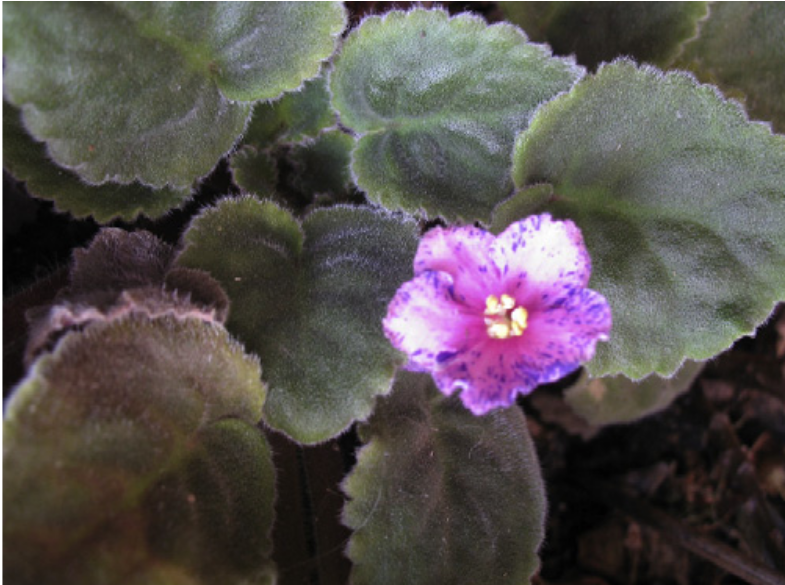
\includegraphics[scale=0.30]{img/5}
\caption{Исходный рисунок}
\end{figure}

\end{frame}

%------------------------------------------------

\begin{frame}
\frametitle{Синхронизация и зрительное внимание}

Рисунок 6 показывает выбор 300 случайных осцилляторов (пикселей) из изображении так, что первые 150 строк соответствуют "лисам" а других 150 линий соответствуют "цветку".

\begin{figure}
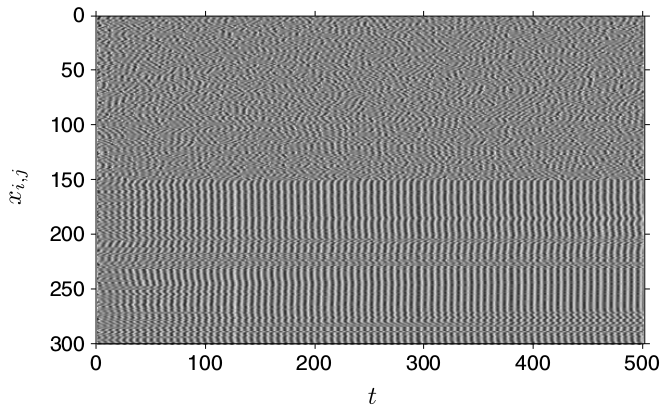
\includegraphics[scale=0.32]{img/6}
\caption{Выбор 300 случайных пикселей}
\end{figure}
\end{frame}

%------------------------------------------------

\begin{frame}
\frametitle{Синхронизация и зрительное внимание}

Рисунки 7 и 8 показывают, что фазовая синхронизация происходит среди осцилляторов, представляющих объект "цветок", в то время как не фазовая синхронизация среди других осцилляторов не наблюдается.

\begin{figure}
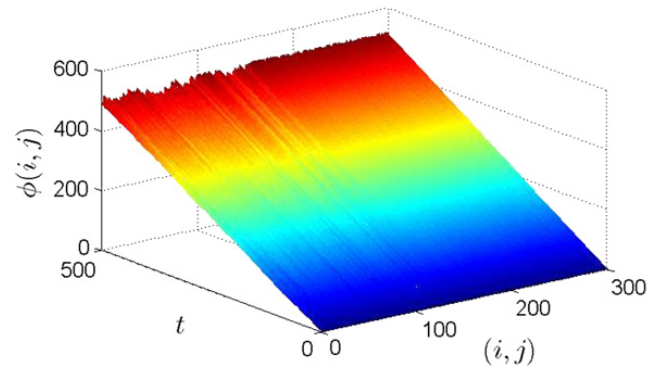
\includegraphics[scale=0.35]{img/7}
\caption{фазовая синхронизация происходит среди осцилляторов}
\end{figure}

\end{frame}

%------------------------------------------------

\begin{frame}
\frametitle{Синхронизация и зрительное внимание}

Рисунки 7 и 8 показывают, что фазовая синхронизация происходит среди осцилляторов, представляющих объект "цветок", в то время как не фазовая синхронизация среди других осцилляторов не наблюдается.

\begin{figure}
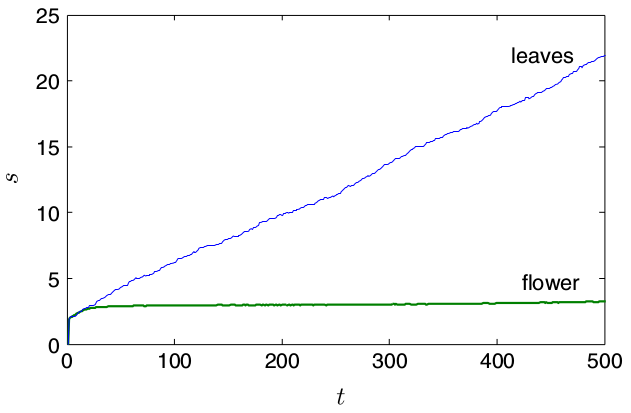
\includegraphics[scale=0.35]{img/8}
\caption{Фазовая синхронизация среди других осцилляторов не наблюдается}
\end{figure}

\end{frame}

%------------------------------------------------

\begin{frame}
\frametitle{Синхронизация и зрительное внимание}

Теперь проведём эксперимент с использованием механизма переключения, чтобы изменить фокус внимания с одного объекта на другой.
На рисунке 9 мы видим искусственное изображение с двумя спиралями. Свободные параметры устанавливаются следующим образом: $\sigma = 0,3$ и $\Delta_w = 0,2$.

\begin{figure}
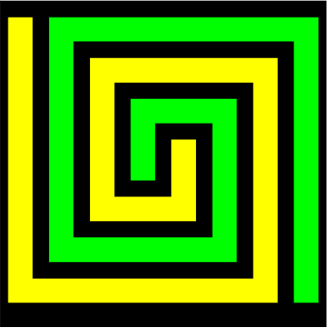
\includegraphics[scale=0.35]{img/9}
\caption{Исходный рисунок второго эксперимента}
\end{figure}

\end{frame}

%------------------------------------------------

\begin{frame}
\frametitle{Синхронизация и зрительное внимание}

Рисунок 10 показывает поведение 150 случайно выбранных осцилляторов (пикселей) от каждого объекта, где каждая строка соответствует осциллятора. Из ряда с 1 по 150, мы можем видеть, что осцилляторы, соответствующие желтому объекта являются первой группой, которая по фазе синхронизирована. Через некоторое время она теряет синхронизацию и возникает фазовая синхронизация второй группы (линии 151 300).

\begin{figure}
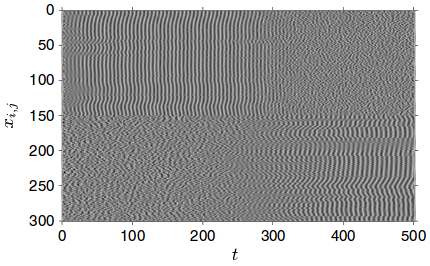
\includegraphics[scale=0.35]{img/10}
\caption{Возникает фазовая синхронизация второй группы}
\end{figure}

\end{frame}

%------------------------------------------------

\begin{frame}
\frametitle{Синхронизация и зрительное внимание}

Рисунок 11 показывает стандартные отклонения фазы роста двух групп осцилляторов.

\begin{figure}
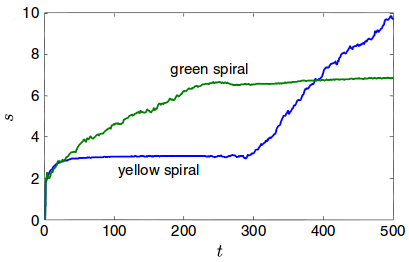
\includegraphics[scale=0.35]{img/11}
\caption{Стандартные отклонения фазы роста двух групп осцилляторов}
\end{figure}

\end{frame}

%------------------------------------------------
\section{Заключение}
%------------------------------------------------

\begin{frame}
\frametitle{Заключение}

Колебательные сети были использованы для решения задач:
\begin{itemize}
\item сегментации изображений,
\item слуховой сегрегации сигнала,
\item функций привязки,
\item выбора объекта.
\end{itemize}
\medskip

Этот вид моделей требует двух механизмов:
\begin{itemize}
\item синхронизация каждого объекта с группой  
\item десинхронизация, чтобы отличить один объект от другого
\end{itemize}
\end{frame}
%------------------------------------------------

\begin{frame}
\frametitle{Заключение}

Сеть осцилляторов имеет явное достоинство - легкость синхронизации группу осцилляторов. Но есть и недостатки, связанные с разделением разных объектов, у которых случайно совпали траектории синхронизации.
\medskip

Возможны следующие возможные направления  ее дальнейшей разработки:
\begin{itemize}
\item испытание новых видов сетевого связывания;
\item разработка методов сегментации движущихся изображений;
\item распространение метода на задачи сегментации цветных изображений;
\item развитие подходов к моделированию активного зрения.
\end{itemize}
\end{frame}
%------------------------------------------------
\section{Ссылки}
%------------------------------------------------

\begin{frame}
\frametitle{Ссылки}

\begin{itemize}
\item F.A. Breve, L. Zhao, M.G. Quiles,  and E.E.N. Macau, "Chaotic phase synchronization and desynchronization in an oscillator network for object selection";presented at Neural Networks, 2009, pp.728-737.
\item Антон Конушин, Компьютерное зрение. http://courses.graphicon.ru/main/vision.
\item Кузьмина М.Г., Маныкин Э.А., Сурина И.И. Осцилляторная сеть с управляемой синхронизацией и динамический метод сегментации изображений // Научная сессия МИФИ-2004. Ч.1 Нейроинформатика-2004. 6 Всероссийская научно-техническая конференция. Теория нейронных сетей 1. Нейробиология. Применение нейронных сетей 1, стр. 29-37
\item Иванченко И.В., Шалфеев В.Д. Информационная динамика сложных осцилляторных систем. Учеб. метод. пособие. — Н. Новгород: Изд-во ННГУ, 2006. — 113 с.
\end{itemize}\end{frame}

%------------------------------------------------
\section{Вопросы}
%------------------------------------------------

\begin{frame}
\Huge{\centerline{Вопросы?}}
\end{frame}

%----------------------------------------------------------------------------------------

\end{document} 
